\documentclass[twocol]{ametsoc}
\journal{mwr}

\usepackage{xcolor}
\usepackage{amsmath}
\usepackage{mathtools}
\usepackage{siunitx}

\bibpunct{(}{)}{;}{a}{}{,}

\title{Comparison of Terrain Following and Cut Cell Grids with a Non-Hydrostatic Model}
\authors{James Shaw\correspondingauthor{Dept., Institution, Address, City, State/Country.}}
\affiliation{}
\email{j.shaw@pgr.reading.ac.uk}

\abstract{Enter the text of your abstract here.}

\begin{document}
\newcommand{\TODO}[1]{\textcolor{purple}{TODO: \emph{#1}}}

\maketitle

\TODO{Builds on the work of \citet{schaer2002}, \citet{klemp2011}, \citet{weller-shahrokhi2014} (all MWR) \\
Results also compared with \citet{melvin2010} (QRJ), maybe zaengl2012 (MWR), \citet{good2014} (Atmos Sci Letters)}

\section{Introduction}
Representing orography in numerical weather prediction systems is necessary to model downslope winds and local precipitation patterns.  Terrain also affects global circulation, giving rise to planetary and gravity waves.

There are two main approaches to represent orography on a grid.  With terrain following (TF) layers the terrain's influence decays with height: the bottommost layers follow the underlying surface closely while the uppermost layers are flat.  TF layers are usually implemented on a rectangular computational grid using transformed coordinates.

It is well-known that TF coordinates perform badly in the presence of steep orography: as model resolution increases, steeper gradients lead to larger truncation errors in calculating the horizontal pressure gradientwhich result in spurious winds \citep{dempsey-davis1998} \TODO{or steppeler2002}.  Much work has been done to reduce error associated with TF coordinates: firstly by smoothing the effects of terrain with height \citep{schaer2002,klemp2011} and, secondly, by improving the accuracy in calculating the horizontal pressure gradient itself \citep{klemp2011} \TODO{and zaengl2012?}.

Despite their associated numerical errors, TF coordinates are attractive because their rectangular structure is simple to process by computer, boundary layer resolution can be increased with variable spacing of vertical layers \citep{schaer2002}, and cell sizes remain almost constant \citep{jebens2011}.

Cut cells is an alternative method in which cells that lie entirely below the terrain are removed, and those that intersect the surface are modified in shape so that they more closely fit the terrain.  This modification means that some cells become very small, which can reduce computational efficiency \TODO{(klein2009)}, and several approaches have been tried to alleviate the problem \TODO{(steppeler2002 thin wall approx,yamazaki-satomura2010 cell combining, jebens2011 implicit method in cut cells)}.

Several studies have found that cut cells produce more accurate results when compared to TF coordinates.  Spurious winds seen in TF coordinates are not present and errors do not increase with steeper terrain \citep{good2014}.  A comparison of TF and cut cells using real initial data by \TODO{steppeler2006} found that precipitation patterns, temperature and wind fields were forecast more accurately in the cut cell model.  

\TODO{that's the high-level intro, now onto BTF/SLEVE grids...}  A variety of vertical decay functions have been formulated that make TF layers flatter with height.  \citet{galchen-somerville1975} proposed a basic terrain following (BTF) coordinate defined as \(z = \left( H - h \right) \left( z^\star / H \right) + h\) where, in two dimensions, \(z(x, z^\star)\) is the height of the coordinate surface at level \(z^\star\), \(H\) is the height of the domain, and \(h(x)\) is the height of the terrain surface.

The smooth level vertical (SLEVE) coordinate proposed by \citet{schaer2002} achieves a more regular TF grid in the middle and top of the domain.  The terrain height is split into large-scale and small-scale components, \(h_1\) and \(h_2\), such that \(h = h_1 + h_2\), with each component having a different exponential decay. The transformation is defined as \(z = z^\star + h_1 b_1 + h_2 b_2\), where the vertical decay functions are given by
\begin{displaymath}
	b_i = \frac{\sinh \left( \left( H - z^\star \right) / s_i \right)}{\sinh \left( H / s_i \right)}
\end{displaymath}
with \(s_1\) and \(s_2\) are the scale heights of large-scale and small-scale terrain respectively.

\TODO{say what we're going to do in this paper}

\TODO{final para of intro: in section 2, section 3 etc etc}

\begin{itemize}
	\item Comparing results BTF, SLEVE and cut cell style grid for three standard two-dimensional test cases
	\item TF grids often shown to have lesser accuracy than cut cells in some test cases, often significantly so.  Our results demonstrate that accuracy need not be much reduced and can even be better than cut cells. \TODO{this is too confrontational!}
\end{itemize}

\section{Results}
\begin{itemize}
	\item \TODO{How much do I need to say about the model?  -- Give a summary: what equation set? finite volume with curl-free pressure grad; lorenz grid; advection scheme}
	\item \TODO{Explain how SnapCol grid is constructed?}
\end{itemize}

\subsection{Advection}
\begin{itemize}
	\item Motivation: tests advection scheme accuracy, especially with grid distortions
	\item Specify domain, terrain, discretisation in time and space, tracer
	\item Specify wind field, projection method for non-divergence
	\item Advection equation in flux form
	\item Upwind-biased cubic advection scheme, non-monotonic, not flux corrected
	\item d/dt scheme (RK2)
\end{itemize}

We compare the following grids:
\begin{itemize}
	\item No orography (which tells us how good the model can get)
	\item BTF
	\item SLEVE (only briefly since it's not adding so much to our argument)
	\item SnapCol (briefly because it's the same as noOrography)
\end{itemize}

\TODO{should we just compare cubicUpwindCPCFit with Sch\"ar's 4th order?  We could also compare our skewCorrected linear with Sch\"ar's linear but I'm not sure what value it would have...}

\begin{figure}
	\centering
	\includegraphics{../msc-publication-fig-advection-tracer/fig-advection-tracer.pdf}
%
	\caption{Horizontally advected tracer contours at $t = \SI{0}{\second}$, \SI{5000}{\second} and \SI{10000}{\second}.  \TODO{identify subfigures}  Contour intervals are every 0.1.}
	\label{fig:advection-tracer}
\end{figure}

Analysis:
\begin{itemize}
	\item Upwind-biased cubic is qualitatively better than Sch\"ar's 4th order leapfrog on BTF grid (figure~\ref{fig:advection-tracer})
	\item SnapCol error, min and max is almost identical to noOrography (unsurprisingly) (table~\ref{tab:advection})  This agrees with \citet{good2014}
	\item SLEVE error, min and max are part-way between BTF and noOrography (again, unsurprisingly)
	\item noOrography, BTF and SLEVE min and max comparable to \citet{schaer2002}
	\item Conclusion: advection more accurate on more regular grids, but nevertheless satisfactory on all grids
\end{itemize}


\begin{figure}
	\centering
	\includegraphics{../msc-publication-fig-advection-error/fig-advection-error.pdf}
	%
	\caption{Errors in horizontal tracer advection at $t = \SI{10000}{\second}$.  \TODO{identify subfigures}  Contour intervals are every 0.01 with negative contours denoted by dashed lines.}
	\label{fig:advection-error}
\end{figure}


\subsection{Resting atmosphere}

\begin{itemize}
	\item Motivation: challenge accuracy of H operator (\TODO{if we mention H op here we'll have to explain it beforehand})
	\item Specify domain, thermodynamics, discretisation in time and space
\end{itemize}

Analysis:
\begin{itemize}
	\item Spurious $w$ significantly less than those found by \citet{klemp2011} for BTF: \SI{0.35}{\meter\per\second} vs \SI{10}{\meter\per\second}
	\item SnapCol $w$ (\SI{1e-3}{\meter\per\second}) significantly than BTF or SLEVE
	\item \TODO{Could also compare with zaengl2012, \citet{good2014}?}
	\item Conclusion: non-orthogonality is a significant cause of numerical error in this test but, again, satisfactory on all grids
\end{itemize}

\begin{figure*}
	\centering
	\includegraphics{../msc-publication-fig-resting/fig-resting.pdf}
%
	\caption{Maximum spurious vertical velocity $w$ in the resting atmosphere test \TODO{identify subfigures}.  Note that vertical scales differ.}
	\label{fig:resting}
\end{figure*}

\subsection{Gravity waves}
\begin{itemize}
	\item \TODO{Motivation: it models a real dynamic process?}
	\item Specify domain, thermodynamics, prescribed inlet wind
	\item Specify sponge layers, BCs
	\item Compare BTF, SLEVE and SnapCol results (SLEVE only briefly as visually identical to BTF)
\end{itemize}

Analysis:
\begin{itemize}
	\item $w$ contours visually similar on all grids, agree with \citet{melvin2010} (Figure~\ref{fig:gw-w})
	\item \TODO{don't know if divergence is relevant -- it's greater on the SnapCol grid (MSc dissertation Figure 4.15e)}
	\item $\theta$ anomalies similar on all grids EXCEPT...
	\item ... on SnapCol grid in lee of mountain near the ground. (Figure~\ref{fig:gw-theta})
	\item \TODO{worth mentioning implications of this?  1. reduced stability, although not enough to create vertical motion in this instance 2. model has no viscosity so thermal mixing should not occur in theory}
	\item Lorenz computation mode has been excited because Exner sample line at $x = \SI{50}{\kilo\meter}$ is in hydrostatic balance (Figure~\ref{fig:gw-exner-theta})
	\item \TODO{We can speculate on what excites the computational mode, but perhaps better not to?}
	\item Little/no evidence of small cell problem -- \TODO{don't know that we can say much here without another vertical momentum test; our hypothesis about the quasi-horizontal flow isn't backed up with a test case}
	\item Conclusion: results similar on all grids, agree with literature, except for Lorenz computational mode on SnapCol grid
\end{itemize}

\begin{figure}
	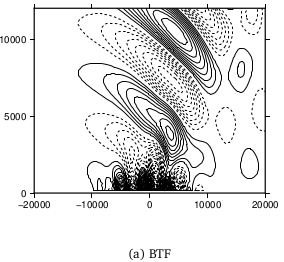
\includegraphics[height=2in]{gw-w-btf.png}
	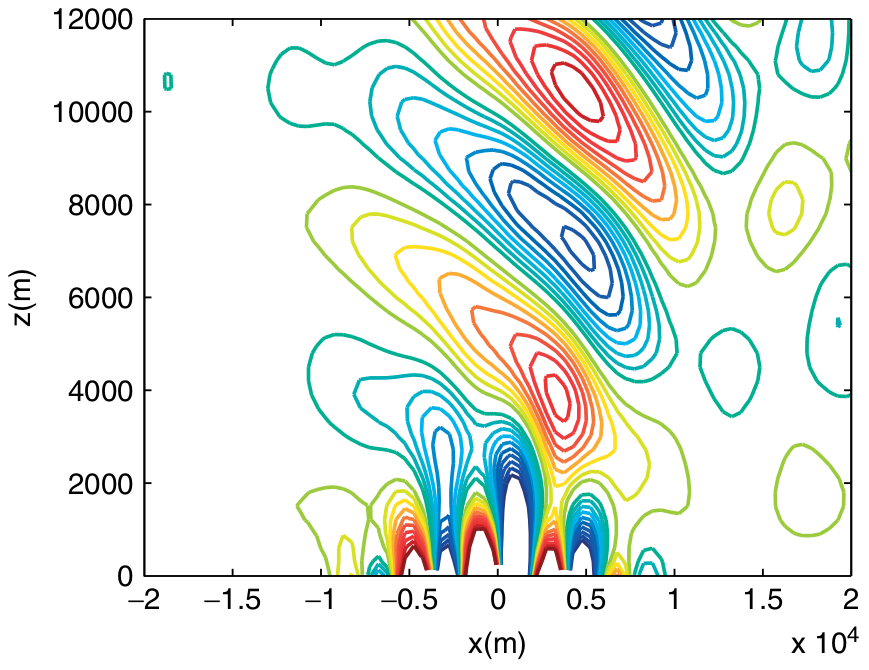
\includegraphics[height=2in]{melvin-7a.png}
%
	\caption{Gravity wave vertical velocities and thermal anomalies from initial thermal profile}
	\label{fig:gw-w}
\end{figure}

\begin{figure}
	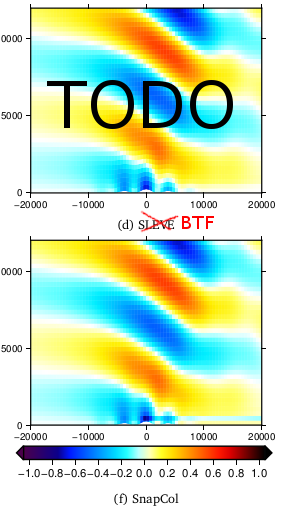
\includegraphics[height=3in]{gw-theta.png}
	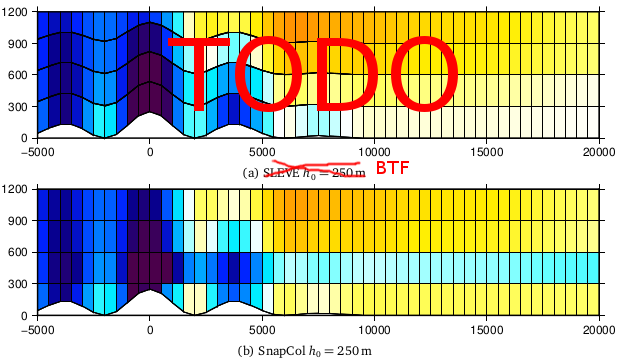
\includegraphics[height=2in]{gw-theta-zoom.png}
%
	\caption{Gravity wave thermal anomalies from initial thermal profile}
	\label{fig:gw-theta}
\end{figure}

\begin{figure}
	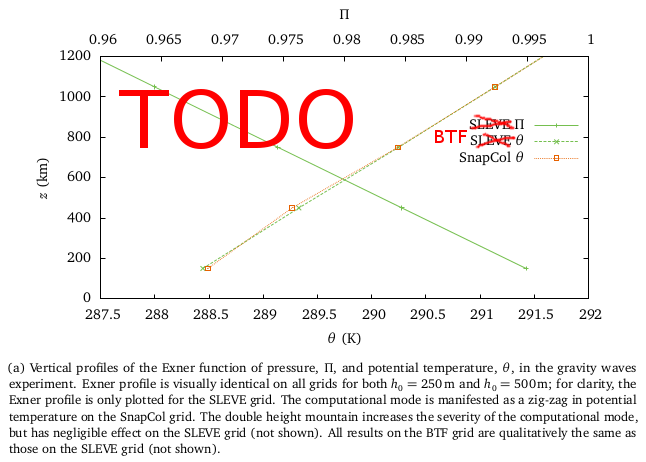
\includegraphics[height=2in]{gw-exner-theta.png}
%
	\caption{Vertical sample line of Exner function of pressure and theta to demonstrate Lorenz computational mode}
	\label{fig:gw-exner-theta}
\end{figure}


\section{Conclusions}
\begin{enumerate}
	\item BTF grid isn't as bad as people say it is.  We found that:
	\begin{itemize}
		\item Upwind-biased cubic advection scheme accurately advects a tracer in non-divergent flows (Figure~\ref{fig:advection-tracer}, \ref{fig:advection-error}, Table~\ref{tab:advection})
		\item spurious vertical velocities are small in resting atmosphere (Figure~\ref{fig:resting})
		\item gravity waves results visually as good as reference solution from \citet{melvin2010} (figure~\ref{fig:gw-w})
	\end{itemize}

	\item Cut cell grids can be worse than TF grids:
	\begin{itemize}
		\item Lorenz computational mode found on SnapCol grid only (figure~\ref{fig:gw-theta}, \ref{fig:gw-exner-theta})
	\end{itemize}

	\item Cut cell grids can also be better than TF grids in more artificial test cases:
	\begin{itemize}
		\item SnapCol $w$ two orders of magnitude smaller in resting atmosphere test
		\item SnapCol advection test as good as noOrography
	\end{itemize}
\end{enumerate}

\textbf{With the exception of the Lorenz computational mode on the SnapCol grid in the gravity waves test, results were satisfactory across BTF, SLEVE and SnapCol grids in all three test cases.}

Miscellany:
\begin{itemize}
	\item Advection accuracy depends on alignment of the flow with grid layers (\TODO{we kinda need wobblyTracerAdvection to reach this conclusion})
\end{itemize}

\section{Further work}
\begin{itemize}
	\item Lorenz computational mode motivates formulation of C-P staggering for cut cell grids
	\item Find out what excites the Lorenz computational mode
	\item \TODO{anything else?}
\end{itemize}

\acknowledgments
Start acknowledgments here.

% REFERENCES

\bibliographystyle{ametsoc2014}
\bibliography{references}

% TABLES

\begin{table}[t]
\caption{Min, max and error norms compared with \citet{schaer2002}}
\label{tab:advection}
%
\begin{center}
\begin{tabular}{ l l l l l l }
\hline\hline
& \multicolumn{3}{c}{Cubic upwind-biased} & \multicolumn{2}{c}{Sch\"ar 4th order} \\
& $\ell^2$ error & min & max & min & max \\
\hline
Analytic  & 0 & 0 & 1 & \multicolumn{1}{c}{---} & \multicolumn{1}{c}{---} \\
BTF 	  & TODO & TODO & TODO & \num{-0.058} & \num{1.001} \\
SnapCol   & TODO & TODO & TODO & \multicolumn{1}{c}{---} & \multicolumn{1}{c}{---} \\
noOrography & TODO & TODO & TODO & \num{-0.002} & \num{0.984} \\
\hline
\end{tabular}
\end{center}
\end{table}

% FIGURES

\end{document}
